% !TEX encoding = UTF-8 Unicode
% !TEX TS-program = pdflatexshell

\documentclass[../main/main.tex]{subfiles}

\begin{document}
\section{Homework}

20 de septiembre: entrega de problemas 1.2(e,f), 1.3 y 1.6 (un único documento pdf)
\subsection*{Problem 1.2.e.}

\begin{align*}
\int _{-\infty}^{\infty}f(x) \delta (x^{2} - a^{2}) d x  &= \\
\textrm{(\small since $x^{2'} = 2x$ and $x=\pm a$ are the poles)}
	&= \int _{-\infty}^{\infty}f(x)\left( \frac{\delta (x-a)}{|2x|} + \frac{\delta(x+a)}{|2x|}\right) d x\\
\textrm{(\small evaluating the distribution)}
	&=\frac{f(a)}{|2a|} + \frac{f(-a)}{|2a|}\\
\textrm{(\small simplifying)}
	&= \frac{f(a) + f(-a)}{|2a|}\\ \qed
\end{align*}

\subsection*{Problem 1.2.f.}

\begin{align*}
\int _{-\infty}^{\infty}f(x) \left[\delta(x-a) - \delta(x+a)\right]d x  &= \\
\textrm{(\small evaluating and simplifying)}
	&=f(a) - f(-a) \\
	\qed
\end{align*}

\pagebreak
\subsection*{Problem 1.3}

Draw a squema of

\begin{align*}
e^{-x^{2}/4}\left(\comb_{1}(x) + comb_{1.5}(x)\right)&\\
&=e^{-x^{2}/4}\sum_{n=-\infty}^{\infty}\left(\delta(x-n) +\delta(x-1.5n)\right)
\end{align*}

Therefore, this is a discretized function, where the pole size is proportional to the gaussian  $e^{-x^{2}/4}$ on all integers and multiples of $1.5n$ except in those integers in which both conditions are met (the multiples of 3), the pole size is twice that of the gaussian instead.

In the following drawing those that get a double contribution are marked in red and the heights of the arrows represent the pole weight.

\begin{center}
	\pgfmathsetmacro{\h}{1}
	\pgfmathsetmacro{\k}{0.3}
	\pgfmathsetmacro{\T}{1}
	\pgfmathsetmacro{\Tminusk}{\T-\k}
    \begin{tikzpicture}[x=1cm, y=2cm]
    % grid
	\draw[help lines, dotted] (-4,-1) grid (4, 3);
        \draw[thin](-4,0)--(4,0);
        \draw[thin](0,-1)--(0,3);
        \foreach \x [evaluate={\hval=exp(-(3*\x-1)*(3*\x-1)/4)}] in {-1, ..., 1} {
		\draw[->, very thick] (3*\x-1, 0) --+(0, \hval) ;
        };
         \foreach \x [evaluate={\hval=exp(-(3*\x+1)*(3*\x+1)/4)}] in {-1, ..., 1} {
		\draw[->, very thick] (3*\x+1, 0) --+(0, \hval) ;
        };
        \foreach \x [evaluate={\hval=exp(-\x*\x/4*9)}] in {-1, ..., 1} {
		\draw[->, very thick, red] (3*\x, 0) --+(0, 2*\hval) ;
        };
        \foreach \x [evaluate={\hval=exp(-(3*\x+1.5)*(3*\x+1.5)/4)}] in {-2, ..., 1} {
		\draw[->, very thick] (3*\x+1.5, 0) --+(0, \hval) ;
        };

        	\draw [|<->|] (0,-0.05)
		--++(1,0) node[pos=0.5, anchor = north] {+1n};
        	\draw [|<->|] ++(0,-0.3)
		--++(1.5,0) node[pos=0.5, anchor = north] {+1.5n};

	\draw [|<->|] ++(0,-0.6)
		--++(+3,0) node[pos=0.5, anchor = north] {+3n};


    \end{tikzpicture}
\end{center}

\subsection*{Problem 1.6}

Express the following signal as a Fourier series in 3 different ways.

NOTE: No entiendo que quiere decir con ``de tres formas distintas''. ?`Quiere decir calcularlo de tres formas distintas? Lo he calculado de una vez de forma general. Luego lo he interpretado en codigo, y he escrito una forma específica, no se si eso es a lo que se refería.

\begin{center}
	\pgfmathsetmacro{\h}{1}
	\pgfmathsetmacro{\k}{0.5}
	\pgfmathsetmacro{\T}{1}
	\pgfmathsetmacro{\Tminusk}{\T-\k}
    \begin{tikzpicture}
    % grid
	\draw[help lines, dotted] (-3,1)  node[thick] {$f(x)$} grid (3, -2);
        \draw(-3,0)--(3,0);
        \draw(0,-1)--(0,2);
     % drawing
     % This can be more clean with \foreach \x in {0, ... , 5} homework for the reader
     	\draw[very thick] (-3+\k/2, 0) --
                ++(\Tminusk, 0)  node(abelow){} --
                ++(0, \h) node (a){} --
                ++(\k, 0) node(b){} --
                ++(0, -\h) --
                ++(\Tminusk, 0)  node(bbelow){}--
                ++(0, \h) --
                ++(\k, 0) --
                ++(0, -\h) --
                ++(\Tminusk, 0) --
                ++(0, \h) --
                ++(\k, 0) --
           		++(0, -\h) --
                ++(\Tminusk, 0) --
                ++(0, \h) --
                ++(\k, 0) --
                ++(0, -\h) --
		        ++(\Tminusk, 0) --
                ++(0, \h) --
                ++(\k, 0) node(c){} --
                ++(0, -\h) node(d){} --
		(3, 0);
	\draw [|<->|] (a.north) --(b.north) node[pos=0.5, anchor = south] {k};
	\draw [|<->|] (abelow.south) --(bbelow.south) node[pos=0.5, anchor = north] {T};
	\draw [|<->|] (c.east) --(d.east) node[pos=0.5, anchor = west] {h};

	\filldraw[blue]  (-\k/2, \h) circle (1.7pt) node[anchor=south east] (P) {$(-\frac k2, h)$};
	\filldraw[red]  (\k/2, \h) circle (1.7pt) node[anchor=south west] (P) {$(\frac k2, h)$};
	\filldraw[blue]  (-\T/2, 0) circle (1.7pt) node[anchor=north] (P) {$(-\frac T2, 0)$};
	\filldraw[red]  (\T/2, 0) circle (1.7pt) node[anchor=north west] (P) {$(\frac T2, 0)$};

    \end{tikzpicture}
\end{center}



	We can calculate
	\begin{align*}
	a_{0} &= \frac{1}{T} \fourier[-T/2][T/2]{f(x)} \\
	a_{n} &= \frac{2}{T} \fourier[-T/2][T/2]{f(x) \cos\left(\frac{2\pi n}{T} y\right)} \\
	b_{n} &= \frac{2}{T} \fourier[-T/2][T/2]{f(x) \sin\left(\frac{2\pi n}{T} y\right)}
	\end{align*}

	Such that

		\begin{equation*}
	f(x) = a_{0} + \sum_{n=1}\left(a_{n} \cos ( 2\pi \nu n x) + b_{n} \sin( 2\pi \nu n x)\right)
	\end{equation*}


	Firstly, trivially, $a_{0}=\frac{kh}{T}$ and $b_{n} = 0,$ since the function is even.
	Then,

	\begin{align*}
	a_{n} &= \frac{2h}{T} \fourier[-k/2][k/2]{ \cos\left(\frac{2\pi n}{T} y\right)} \\
		&= \frac{\cancel{2}h}{\cancel{T}}\frac{1}{\frac{\cancel{2}\pi n}{\cancel{T}}}\left( 2\sin\left(\frac{\cancel{2}\pi n}{T} \frac{k}{\cancel{2}}\right)  \right)\\
		&= \frac{2h}{\pi n} \sin\left(\frac{\pi n k}{T} \right)
	\end{align*}

	Now, in our case, $2 = \frac T k$, therefore

	\begin{equation*}
	a_{n} = \frac{2h}{\pi n} \sin\left(\frac{\pi n }{2} \right) =
	\begin{cases}
	\textrm{if $n=2m$ } & \frac{2h}{\pi n} \sin\left(\pi m  \right) = 0\\
	\textrm{if $n=2m-1$} &\frac{2h}{\pi n} \sin\left(\pi m - \frac \pi 2\right) = (-1)^{m+1}\frac{2h }{\pi n}
	\end{cases}
	\end{equation*}

	\begin{equation*}
	\boxed{
		F(x) = \frac{h}{2} -
			\sum_{m=1}(-1)^{m}\frac{2h }{\pi (2m-1)}
				\cos\left(\frac{\pi (2m -1)}{T} x \right)
	}
	\end{equation*}

Side-note, verifying at zero, using the typical $\arctan 1$ expansion

	\begin{equation*}
	\frac{F(0)}{h}
	= \frac{1}{2} - \frac 2 \pi \sum_{m=1}\frac{(-1)^{m}}{(2m-1)}
	= \frac{1}{2} + \frac 2 \pi  \frac \pi 4
	= 1
	\end{equation*}

\pagebreak
\begin{center}

\begin{rcode}[Quick software verification in R]
library(tidyverse)
square <- function(x, order=1) {
#  Reference equation F(x) = 1/2 -
#    \sum_{m=0}(-1)^{m}\frac{2h }{\pi (2m-1)} \cos(\frac{\pi (2m -1)}{T} x )
  r <- 1/2
  for (o in seq_len(order)) {
    factor <- (-1)^(o %% 2)*2/(pi* (2*o-1))
    cosine <- cos(pi * ( 2 * o - 1 ) * x)
    r <- r - factor * cosine
  }
  r
}

x <-seq(-2, 2,length.out= 6000)

dat <- tibble(x,
             `order 1`=square(x, order=1),
             `order 2`=square(x, order=2),
             `order 5`=square(x, order=5),
             `order 10`=square(x, order=10),
             `order 100`=square(x, order=100),
)
dat %>%
  pivot_longer(-x) %>%
  ggplot(aes(x=x, y=value)) +
  geom_line(aes(color = name, linetype = name))
\end{rcode}
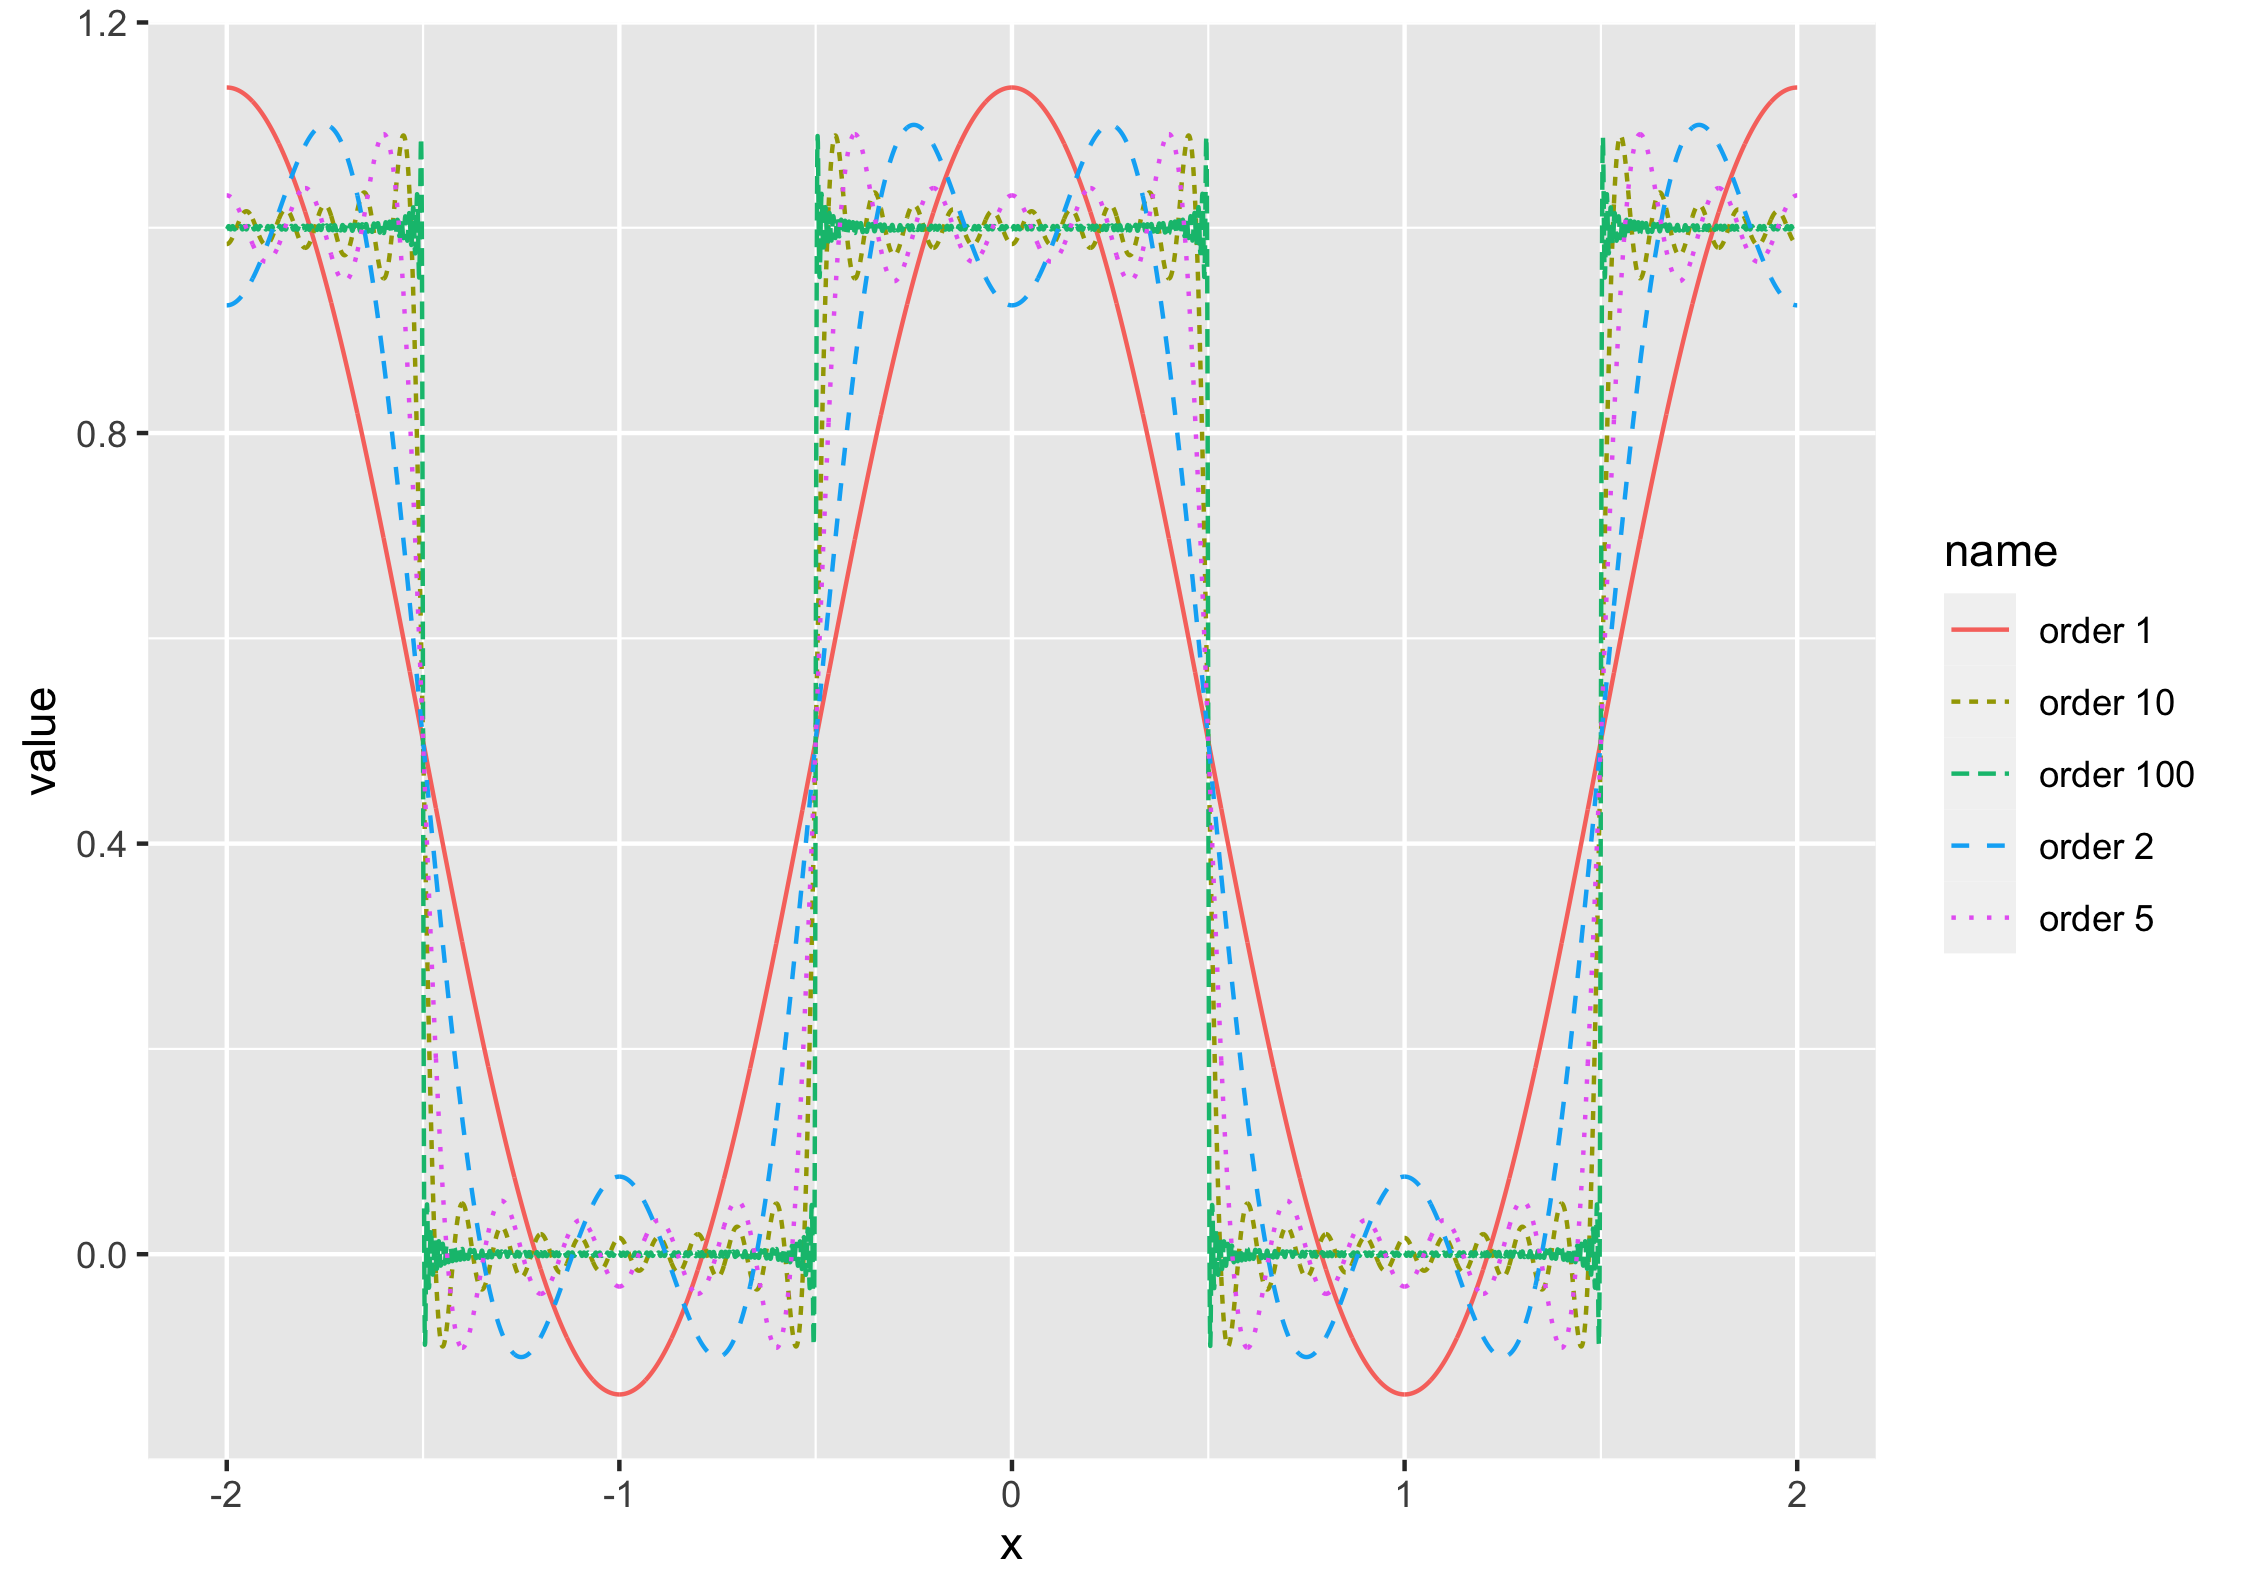
\includegraphics[
	width=0.75\textwidth,
	keepaspectratio,
]{1-1.6-homework-fourier-square.png}
\end{center}


\end{document}
